% ============================================================================
% Panel A / Panel B 图注草稿
% 原先画在图上的参数标注（Panel A 的 N=2e4、Panel B 的 eta=100）已移入此处。
% 标签名沿用占位，接入正文时请改成与 \label{fig:...} 体系一致的名字。
% ============================================================================

% ---------------------------------------------------------------- Panel A ---
\begin{figure}[htbp]
  \centering
  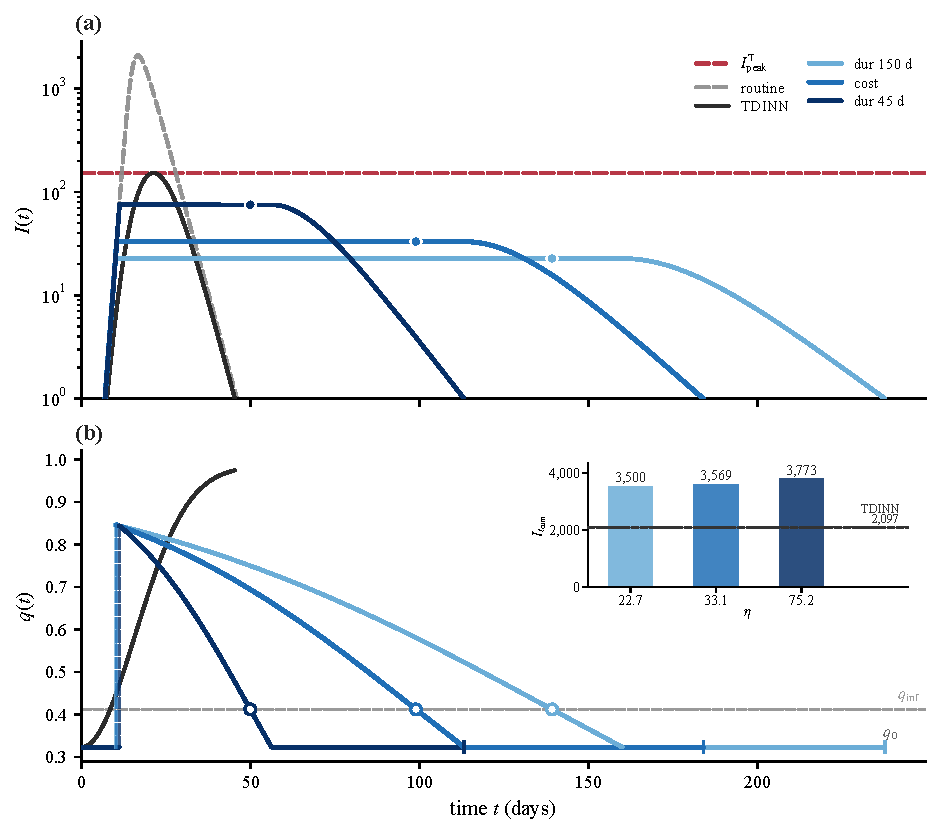
\includegraphics[width=0.85\textwidth]{figures/fig_panel_A.pdf}
  \caption{$\eta$ 杠杆：固定有效人口 $N_{\rm eff}=2\times10^{4}$，沿四条尺度不变
  边界取阈值 $\eta=\theta N_{\rm eff}$ 的情景一阈值控制轨迹。各条平台的高度即其 $\eta$，已在平台下降转角处直接标出；四条边界依次为
  interior（$\Delta t=30$ d，$\theta_{\rm int}=5.612\times10^{-3}$，$\eta=112.2$）、
  dur 45 d（$\theta_{\rm dur45}=3.762\times10^{-3}$，$\eta=75.2$）、
  cost（$\theta_{\rm cost}=1.656\times10^{-3}$，$\eta=33.1$）与
  dur 150 d（$\theta_{\rm dur150}=1.137\times10^{-3}$，$\eta=22.7$）。
  (a) 社区感染者 $I(t)$（对数纵轴）：四条平台分别贴合各自的 $\eta$，且因
  $N_{\rm eff}<N^\ast_{45}$ 全部落在 $I_{\rm peak}^{\rm T}$ 之下（红点线）。
  灰点线为同一 $N_{\rm eff}$ 下的常规控制；黑实线为 TDINN 控制，取西安全市口径下
  的原始拟合轨迹（峰值 $151.90$、清零 $45.27$ d），作为固定的现实参照，不随
  $N_{\rm eff}$ 重算（见第~\ref{sec:dominance}~节 TDINN 基准的口径说明）。
  (b) 隔离率 $q_c(t)$：四条松弛曲线与 TDINN 的上升高斯 $q_{\rm TDINN}(t)$；
  灰点线与灰虚线分别为 $q_0=0.3230$ 与拐点高度 $\qinf=1-1/[2(1-\beta)]=0.4119$。
  白心圆为各条曲线的凹凸拐点，均落在 $\qinf$ 上，与其只依赖 $\beta$、
  不依赖 $(N_{\rm eff},\eta)$ 的结论一致。}
  \label{fig:panel_eta_lever}
\end{figure}

% ---------------------------------------------------------------- Panel B ---
\begin{figure}[htbp]
  \centering
  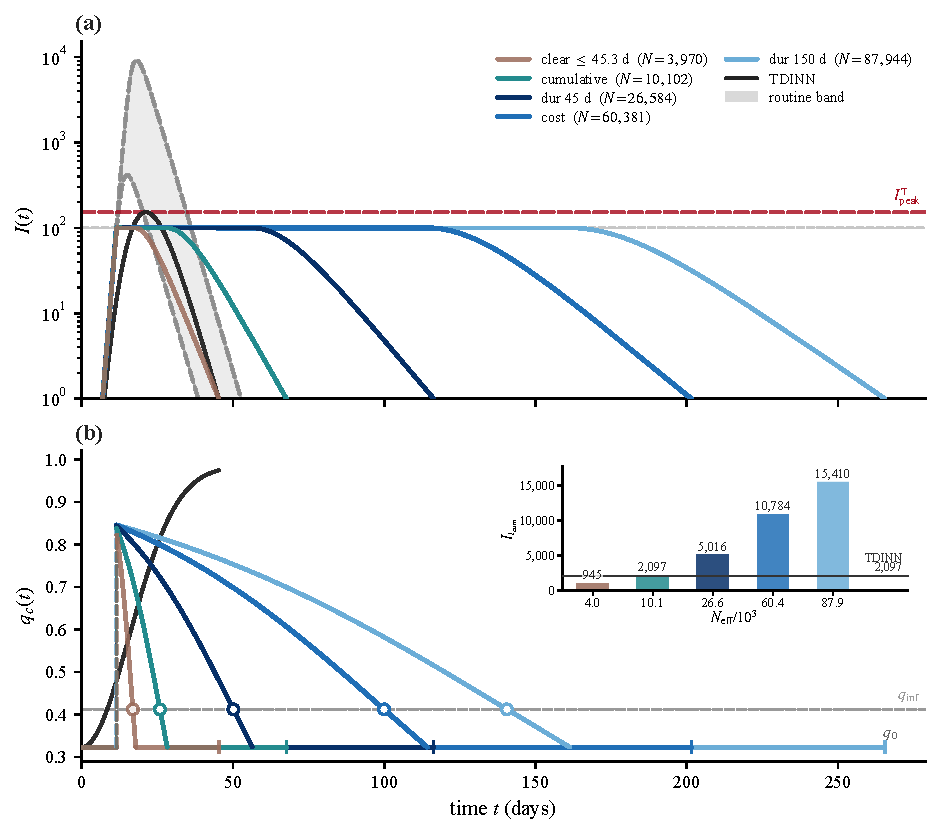
\includegraphics[width=0.85\textwidth]{figures/fig_panel_B.pdf}
  \caption{$N$ 杠杆：固定绝对阈值 $\eta=100$，在六个有效人口下的情景一阈值控制轨迹。
  六条平台高度相同（均为 $\eta$），故 $N_{\rm eff}$ 无法在纵轴上直读，各曲线对应的 $N_{\rm eff}$ 已随角色名列于图例；六个取值取自各条边界与 $\eta=100$ 的交点：
  clear $\le45.3$ d（$N_{\rm eff}=4{,}602$）、cumulative（$10{,}106$）、
  interior（$17{,}819$）、dur 45 d（$26{,}582$）、cost（$60{,}386$）、
  dur 150 d（$87{,}951$）。
  (a) $I(t)$（对数纵轴）：六条平台\emph{全部恒在} $\eta=100$（灰虚线），与池规模无关，
  这是强度量只通过 $\theta=\eta/N_{\rm eff}$ 进入的直接体现；平台\emph{时长}则随
  $N_{\rm eff}$ 增大而显著拉长。灰色带为常规控制在 $N_{\rm eff}\in[4{,}602,\,87{,}951]$（与上列六个取值同范围）
  上取 $8$ 条几何间隔轨迹的逐点最小--最大包络，仅绘制到全部成员均未清零为止；
  两条灰点线为区间端点的代表轨迹，因各成员按自身 $N_{\rm eff}$ 重拟合 $I_0$、轨迹相互交叉，
  端点轨迹并非处处即为包络。带宽即该反事实策略对池规模的敏感度（峰值处上下相差约 $55$ 倍），
  与阈值控制平台的零带宽形成对照。黑实线为 TDINN 控制的西安全市原始拟合轨迹
  （峰值 $151.90$、清零 $45.27$ d）：它是已发生的现实控制，作为固定参照只画一条，
  不随 $N_{\rm eff}$ 重算；红点线为其峰值 $I_{\rm peak}^{\rm T}$。
  (b) $q_c(t)$：六条松弛曲线与 TDINN 的 $q_{\rm TDINN}(t)$；白心圆的拐点同样全部落在
  $\qinf=0.4119$，给出跨 $N_{\rm eff}$ 的不变性，与图~\ref{fig:panel_eta_lever}
  的跨 $\eta$ 不变性互补。}
  \label{fig:panel_N_lever}
\end{figure}
